%%%%%%%%%%%%%%%%%%%%%%%%%%%%%%%%%%%%%%%%%%%%%%%%%%%%%%%%%%%%%%%%%%%%%%%%%%%%%%%%
\documentclass[letterpaper, 10 pt, conference]{ieeeconf}
%\documentclass[a4paper, 10pt, conference]{ieeeconf}

\IEEEoverridecommandlockouts
\overrideIEEEmargins

%\pdfobjcompresslevel=0
%\pdfminorversion=4

\usepackage{graphicx}
\usepackage{amsmath}
\usepackage{array}
\usepackage{booktabs}
\usepackage{multirow}
\usepackage{makecell}
\renewcommand\cellalign{lc}
\usepackage{float}
\floatstyle{plain}
\newfloat{equ}{htbp}{loe}
\floatname{equ}{Equation}
\usepackage{tikz}
\usetikzlibrary{arrows.meta, positioning}
\usepackage{booktabs}
\usepackage{tabularx}
\usepackage{caption}
\captionsetup{compatibility=false, labelfont=bf, labelsep=colon} % set style for compatibility with unknown class
%% colocados Omar:
\usepackage{soul}
\usepackage{xcolor}
\usepackage{subcaption}
%%%%%%%%%%%%%%%%%%%%%%%%%%%%%%%%%%%%%%%%%%%%%%%%%%%%%%%%%%%%%%%%%%%%%%%%%%%%%%%%

\title{\LARGE \bf
Validation of the Theta/Alpha Ratio (Fz/Pz) as an EEG-Based Index of Cognitive Load in Controlled and Ecological Paradigms
}

\author{%
\parbox{\linewidth}{\centering
Edgar R. Hernandez-Rios$^{1,2}$, J. Aparicio-Juarez$^{1}$, Omar A. Dominguez-Ramirez$^{1}$, and Christian Penaloza$^{2,3}$\\
\vspace{1mm}
$^{1}$Universidad Autonoma del Estado de Hidalgo (UAEH), Mexico\\
$^{2}$Mirai Innovation Research Institute, Osaka, Japan\\
$^{3}$Universidad Autonoma de Chihuahua (UACH), Mexico
}\thanks{*This work was supported by Mirai Innovation Research Institute and the Mexican Secretariat of Science, Humanities, Technology, and Innovation (SECIHTI), Mexico.}%
%
}

\newcolumntype{C}{>{\centering\arraybackslash}X}
% Configuración del estilo del título para que sea más estético y compacto
\captionsetup[table]{
  labelfont={bf,small},
  textfont={it,small},
  justification=justified,
  singlelinecheck=false,
  labelsep=period,
  skip=5pt
}
\begin{document}

\maketitle
\thispagestyle{empty}
\pagestyle{empty}

%%%%%%%%%%%%%%%%%%%%%%%%%%%%%%%%%%%%%%%%%%%%%%%%%%%%%%%%%%%%%%%%%%%%%%%%%%%%%%%%
\begin{abstract}
Reliable and interpretable neurophysiological markers of cognitive load are essential for the development of adaptive human--machine interfaces and neuroergonomic systems. This paper validates an EEG-based cognitive load index defined as the ratio of frontal theta power to parietal alpha power (Theta$_{Fz}$/Alpha$_{Pz}$) across two complementary paradigms: a controlled laboratory task and an ecological interactive task. EEG was acquired at 250~Hz using an 8-channel system streamed via Lab Streaming Layer (LSL) and analyzed offline using a standardized preprocessing pipeline including notch and bandpass filtering, spectral estimation via Welch power spectral density, and explicit artifact handling.

In the controlled paradigm, cognitive load was manipulated using passive reading (low demand) and a Stroop interference task (high demand). Six recording sessions met predefined signal-quality criteria and consistently showed higher Theta/Alpha ratios in the high-demand condition, with group-level means increasing from 1.37 (SD=1.80) to 4.65 (SD=4.99) and a paired Cohen’s $d=0.75$. In the ecological paradigm, the same index was normalized to baseline and evaluated during an exergaming task; 6 out of 8 sessions exhibited increased ratios relative to baseline, indicating sensitivity to task engagement while revealing inter-session variability.

Together, these results support the Theta/Alpha ratio (Fz/Pz) as a practical and interpretable index for assessing cognitive load in both controlled and ecological contexts.

In the ecological paradigm, cognitive load was assessed during an exergaming task grounded in human–robotic physical interaction (HRpI), combining voluntary motor exploration and kinesthetic stimulation within a virtual environment imposing sustained attentional demands. This paradigm enabled evaluation of the Theta/Alpha index under interactive and sensorimotor conditions beyond strictly controlled laboratory tasks.


\end{abstract}



\begin{keywords}
EEG, cognitive load, theta/alpha ratio, Stroop task, exergaming, haptic interface, Lab Streaming Layer (LSL).
\end{keywords}


%%%%%%%%%%%%%%%%%%%%%%%%%%%%%%%%%%%%%%%%%%%%%%%%%%%%%%%%%%%%%%%%%%%%%%%%%%%%%%%%
\section{INTRODUCTION}

Quantifying cognitive load from neurophysiological signals is a central challenge in neuroergonomics, adaptive human--machine interaction, and intelligent training systems. Among available sensing modalities, electroencephalography (EEG) has been widely adopted due to its high temporal resolution and its direct relationship with cortical dynamics underlying attention, executive control, and mental effort. In recent years, there has been renewed interest in simple and interpretable EEG-derived indices that can robustly capture variations in cognitive demand across tasks and contexts.

Spectral features in the theta (4--7 Hz) and alpha (8--12 Hz) bands have consistently been linked to cognitive workload. Increases in frontal theta power have been associated with sustained attention, conflict monitoring, and executive control, whereas decreases in parietal alpha power have been related to increased task engagement and information processing demands. Recent studies and meta-analyses have confirmed that these spectral modulations are among the most reliable EEG correlates of cognitive load across experimental paradigms and subject populations~\cite{c1,c4}. Building on this evidence, band power ratios—particularly theta/alpha and alpha/theta ratios—have been proposed as compact indices that integrate complementary neural mechanisms into a single scalar measure of mental workload~\cite{c1,c7}.

Recent work has systematically evaluated the sensitivity and reliability of such ratios, demonstrating that theta-to-alpha and alpha-to-theta indices can discriminate levels of cognitive demand across controlled laboratory tasks and immersive environments~\cite{c1,c2,c3}. Importantly, methodological factors such as electrode configuration, preprocessing choices, and artifact handling have been shown to substantially affect index stability, underscoring the need for clearly defined and reproducible pipelines when validating EEG-based workload metrics~\cite{c4,c6}. These considerations are particularly relevant for applications that aim to deploy cognitive load indices beyond offline analysis, including adaptive systems and real-time monitoring scenarios~\cite{c10}.

Controlled cognitive interference paradigms, such as the Stroop task, remain a standard benchmark for eliciting robust and well-characterized increases in cognitive load. Recent EEG studies have confirmed that Stroop interference reliably induces frontal theta increases and concomitant alpha modulations consistent with elevated executive demand~\cite{c5,c9}. At the same time, there is growing interest in extending cognitive load assessment to more ecological scenarios, including interactive and game-based tasks, where task demands are less structured and subject engagement may vary more substantially across individuals~\cite{c2,c3}.

In this work, we validate a simple and interpretable EEG-based cognitive load index defined as the ratio of frontal theta power (Fz) to parietal alpha power (Pz). The index is evaluated across two complementary paradigms: (i) a controlled laboratory protocol contrasting low cognitive load (passive reading) and high cognitive load (Stroop interference), and (ii) an ecological exergaming task involving different interaction modalities. By applying a common acquisition and processing pipeline with explicit signal-quality criteria, this study aims to assess both the discriminative validity of the theta/alpha ratio under controlled conditions and its sensitivity in a more naturalistic task setting.



%%%%%%%%%%%%%%%%%%%%%%%%%%%%%%%%%%%%%%%%%%%%%%%%%%%%%%%%%%%%%%%%%%%%%%%%%%%%%%%%
\section{METHODS}

\subsection{Participants and Data Overview}
EEG data were collected across two complementary experimental paradigms: a controlled laboratory protocol and an ecological exergaming task. For the controlled paradigm, a total of 14 recording sessions were acquired. Sessions were subsequently evaluated using predefined signal-quality criteria, independently of effect direction. Six sessions satisfied these criteria and were included in the primary controlled analysis. 

For the ecological paradigm, multiple sessions were recorded from several participants performing an exergaming task. Analysis was conducted at the session level, focusing on recordings that contained a clearly defined task segment suitable for baseline comparison. No additional exclusion criteria were applied beyond those inherent to the preprocessing pipeline, and all eligible sessions were reported to ensure transparency.

All procedures were conducted with informed consent was obtained from all participants.

\subsection{EEG Acquisition Hardware and Software}
EEG was recorded using the AURA device, an 8-channel EEG system with a nominal sampling rate of 250~Hz. Signals were streamed in real time using Lab Streaming Layer (LSL). A custom graphical interface implemented in PyQt5 was used to guide the experimental protocols and store the recorded data as CSV files.

Electrodes were positioned according to the international 10--20 system at Fp1, Fp2, F3, Fz (channel 3), F4, P3, Pz (channel 6), and P4. The cognitive load index was computed using theta-band activity from Fz and alpha-band activity from Pz.

\subsection{Offline Preprocessing}
All EEG data were processed offline using a standardized preprocessing pipeline. Signals were notch filtered at 60~Hz (Q~=~30) to attenuate power line interference, followed by bandpass filtering between 1 and 40~Hz using a fourth-order Butterworth filter. 

Common average reference (CAR) was optionally applied depending on the analysis pipeline; CAR was enabled in the ecological paradigm analysis. The effective sampling rate was assumed to be 250~Hz; when required, it can be estimated from timestamps.

\subsection{Spectral Analysis and Cognitive Load Index}
Spectral power was estimated using Welch’s power spectral density (PSD) method. The EEG signal was segmented into windows of 250 samples (1~s at 250~Hz) with 50\% overlap (step size of 125 samples). For each window, theta-band power (4--7~Hz) was computed from channel Fz, and alpha-band power (8--12~Hz) from channel Pz. Bandpower was defined as the integral of the PSD over the corresponding frequency band using the trapezoidal rule.

The cognitive load index was defined for each window as:
\[
\mathrm{Index} = \frac{\Theta_{Fz}}{\alpha_{Pz}}.
\]
Non-finite values were discarded, and division by zero was avoided. The index was averaged across valid windows within each phase or session.

An overview of the complete EEG processing pipeline and the computation of the cognitive load index is summarized in Fig.~\ref{fig:pipeline}.

\begin{figure}[H]
\centering
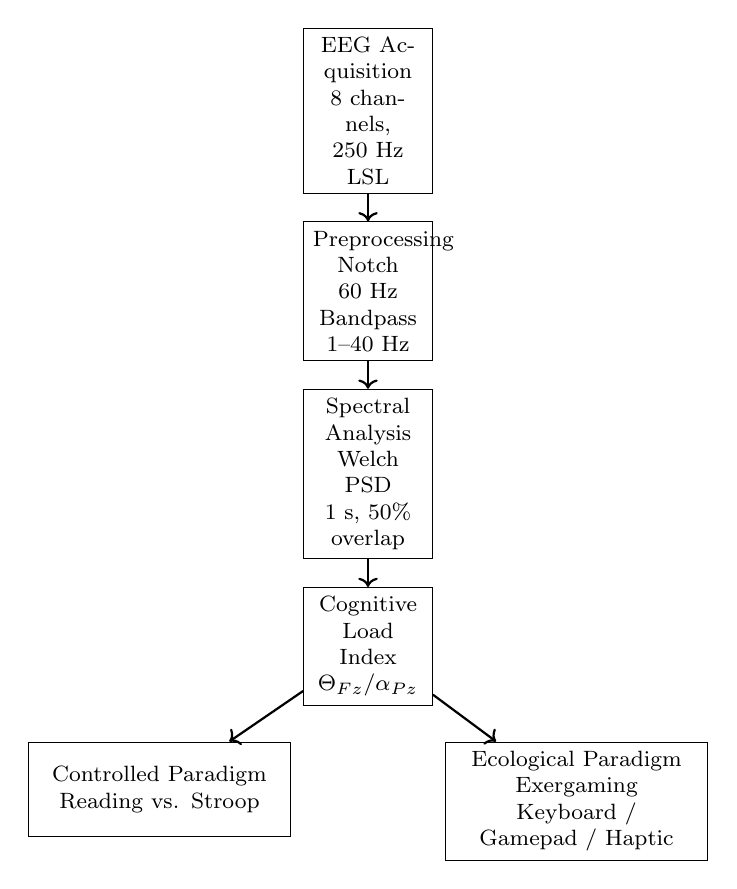
\begin{tikzpicture}[
    block/.style={
        rectangle,
        draw,
        text width=1.4cm,
        align=center,
        minimum height=1.2cm,
        font=\footnotesize
    },
    arrow/.style={->, thick}
]

% Vertical pipeline (compact)
\node[block] (acq) {EEG Acquisition\\
8 channels, 250 Hz\\
LSL};

\node[block, below=0.35cm of acq] (prep) {Preprocessing\\
Notch 60 Hz\\
Bandpass 1--40 Hz};

\node[block, below=0.35cm of prep] (spec) {Spectral Analysis\\
Welch PSD\\
1 s, 50\% overlap};

\node[block, below=0.35cm of spec] (index) {Cognitive Load Index\\
$\Theta_{Fz} / \alpha_{Pz}$};

% Branches (very compact)
\node[block, below left=0.45cm and 0.15cm of index, text width=3.1cm] (controlled)
{Controlled Paradigm\\
Reading vs. Stroop};

\node[block, below right=0.45cm and 0.15cm of index, text width=3.1cm] (ecological)
{Ecological Paradigm\\
Exergaming\\
Keyboard / Gamepad / Haptic};

% Arrows
\draw[arrow] (acq) -- (prep);
\draw[arrow] (prep) -- (spec);
\draw[arrow] (spec) -- (index);
\draw[arrow] (index) -- (controlled);
\draw[arrow] (index) -- (ecological);

\end{tikzpicture}
\caption{EEG processing pipeline and cognitive load index computation. A common acquisition and preprocessing pipeline is followed by paradigm-specific analysis for controlled and ecological tasks.}
\label{fig:pipeline}
\end{figure}
\subsection{Artifact Detection and Window Selection}
Artifacts were detected independently for channels Fz and Pz using three criteria: Z-score threshold (3), interquartile range (IQR) threshold (multiplier of 3), and absolute amplitude threshold (200~$\mu$V). Samples identified as artifacts were handled using linear interpolation; clipping was applied only when too few valid samples remained.

After artifact handling, the cognitive load index was recomputed. Only windows with finite index values within a reasonable range (0.01--100) were retained for analysis.

\subsection{Controlled Paradigm: Low vs. High Cognitive Load}
The controlled paradigm followed a baseline--low--high protocol. After a signal verification phase, participants completed a baseline consisting of 90~s with eyes open followed by 90~s with eyes closed. The low cognitive load condition consisted of passive reading of a text for approximately 3~minutes. The high cognitive load condition consisted of a Stroop color--word interference task of similar duration, in which participants identified the ink color rather than the written word using keyboard inputs (R/B/G/Y).

A session was considered \emph{includable} if, in both low and high load phases, the artifact percentage in Fz or Pz did not exceed 50\% and at least two valid windows remained after cleaning. Among includable sessions, the hypothesis tested was that the mean cognitive load index would be higher in the high-demand condition than in the low-demand condition (High $>$ Low).
\subsection{Subjective Cognitive Load Assessment: NASA-TLX}

Subjective cognitive workload was assessed using the NASA Task Load Index (NASA-TLX), a widely adopted multidimensional questionnaire for evaluating perceived task demand. The NASA-TLX captures workload across six dimensions: Mental Demand, Physical Demand, Temporal Demand, Performance, Effort, and Frustration.

In the controlled paradigm, participants completed the NASA-TLX questionnaire immediately after each task condition (Low Load: passive reading; High Load: Stroop interference). Raw (unweighted) NASA-TLX scores were computed following standard practice, as recommended for small-sample experimental studies, yielding a global workload score for each condition.

For the ecological exergaming paradigm, NASA-TLX data were collected after task completion when available. Due to the exploratory nature of the ecological recordings and variability in session structure, NASA-TLX scores were used primarily for qualitative and correlational comparison with EEG-derived cognitive load indices.

\subsection{Ecological Paradigm: Exergaming Task}
The ecological paradigm involved an exergaming scenario implemented on a robotic platform with multiple interaction modalities, including keyboard, gamepad, and haptic interface. Data files did not include explicit low/high phase labels; instead, task segments were identified using event markers and segmented into pre-task and task periods.

Baseline values for normalization were obtained either from dedicated baseline recordings or, when available, from baseline data recorded for the same participant in the controlled paradigm. For each session, the cognitive load index was computed for the task segment and normalized relative to baseline:
\[
\mathrm{Index}_{\mathrm{norm}} = \frac{\mathrm{Index}_{\mathrm{task}}}{\mathrm{Index}_{\mathrm{baseline}}}.
\]
Normalized values greater than 1 indicate higher cognitive load during the task compared to baseline.

\subsection{Statistical Analysis}
For the controlled paradigm, index values were averaged per session within the low and high cognitive load phases. Group-level descriptive statistics (mean and standard deviation) were computed across includable sessions. Effect size was quantified using paired Cohen’s $d$ computed on session-wise differences (High minus Low). Given the limited sample size, the analysis focused on descriptive statistics and effect size estimation rather than population-level inference.

For the ecological paradigm, results were summarized at the session level by reporting whether the normalized index during the task segment exceeded baseline. No inferential statistics were applied, and inter-session variability was explicitly reported.

For the controlled paradigm, convergent validity between EEG-based cognitive load indices and subjective workload was explored by examining the correspondence between changes in the theta/alpha ratio and NASA-TLX global scores across Low and High conditions. Given the limited sample size, this analysis was descriptive and focused on consistency of directionality rather than inferential correlation testing.


%%%%%%%%%%%%%%%%%%%%%%%%%%%%%%%%%%%%%%%%%%%%%%%%%%%%%%%%%%%%%%%%%%%%%%%%%%%%%%%%
\section{RESULTS}

\subsection{Controlled Paradigm: Low vs. High Cognitive Load}

From a total of 14 recorded sessions, six sessions satisfied the predefined signal-quality inclusion criteria (artifact percentage in Fz or Pz $\leq$ 50\% and at least 2 valid windows after cleaning in both Low and High phases). These includable sessions were used for the primary controlled analysis. At the session level, all included cases exhibited higher mean theta/alpha ratios in the high-demand condition (Stroop interference) than in the low-demand condition (passive reading), consistent with the study hypothesis (High $>$ Low).

Table~\ref{tab:controlled} reports per-session mean theta/alpha ratios for Low and High conditions, the number of valid analysis windows retained after artifact handling, and the maximum artifact percentage across Fz and Pz in each condition. Despite marked inter-session variability in absolute ratio values, the direction of change (High $>$ Low) was consistent across all included sessions.
% Ejemplo dentro de una columna para demostrar el ajuste
\begin{table}[htbp]
\centering
\caption{Per-session summary for the controlled paradigm: mean theta/alpha ratio in Low and High Load, valid windows after cleaning, and maximum artifact percentage (Fz or Pz) in each condition (six sessions satisfying High $>$ Low).}
\label{tab:controlled}
\footnotesize % Mantenemos fuente pequeña para asegurar que quepa todo
\setlength{\tabcolsep}{2pt} % Reducimos un poco el espacio entre columnas

\begin{tabularx}{\columnwidth}{l CCCC}
\toprule
\textbf{Session} & \textbf{Mean Low} & \textbf{Mean High} & \textbf{Valid win (L/H)} & \textbf{Max art. \% (L/H)} \\
\midrule
S1 & 3.94 & 6.69  & 2 / 2   & 2.57 / 2.14 \\
S2 & 0.09 & 0.10  & 2 / 2   & 2.36 / 1.06 \\
S3 & 0.30 & 11.36 & 2 / 2   & 2.96 / 26.51 \\
S4 & 0.10 & 0.43  & 59 / 64 & 16.46 / 10.07 \\
S5 & 0.35 & 0.39  & 2 / 2   & 1.92 / 29.15 \\
S6 & 3.42 & 8.97  & 2 / 2   & 7.04 / 4.03 \\
\bottomrule
\end{tabularx}
\end{table}

Session identifiers (S1--S6) correspond to the six includable sessions analyzed in the controlled paradigm.

At the group level, the mean theta/alpha ratio increased from 1.37 (SD = 1.80) during Low Load to 4.65 (SD = 4.99) during High Load, yielding a mean difference (High $-$ Low) of 3.29. The corresponding paired Cohen's $d$ computed on session-wise differences was 0.75, indicating a medium effect size. Fig.~\ref{fig:bars} shows the Low vs. High comparison for each included session.

\begin{figure}[H]
\centering
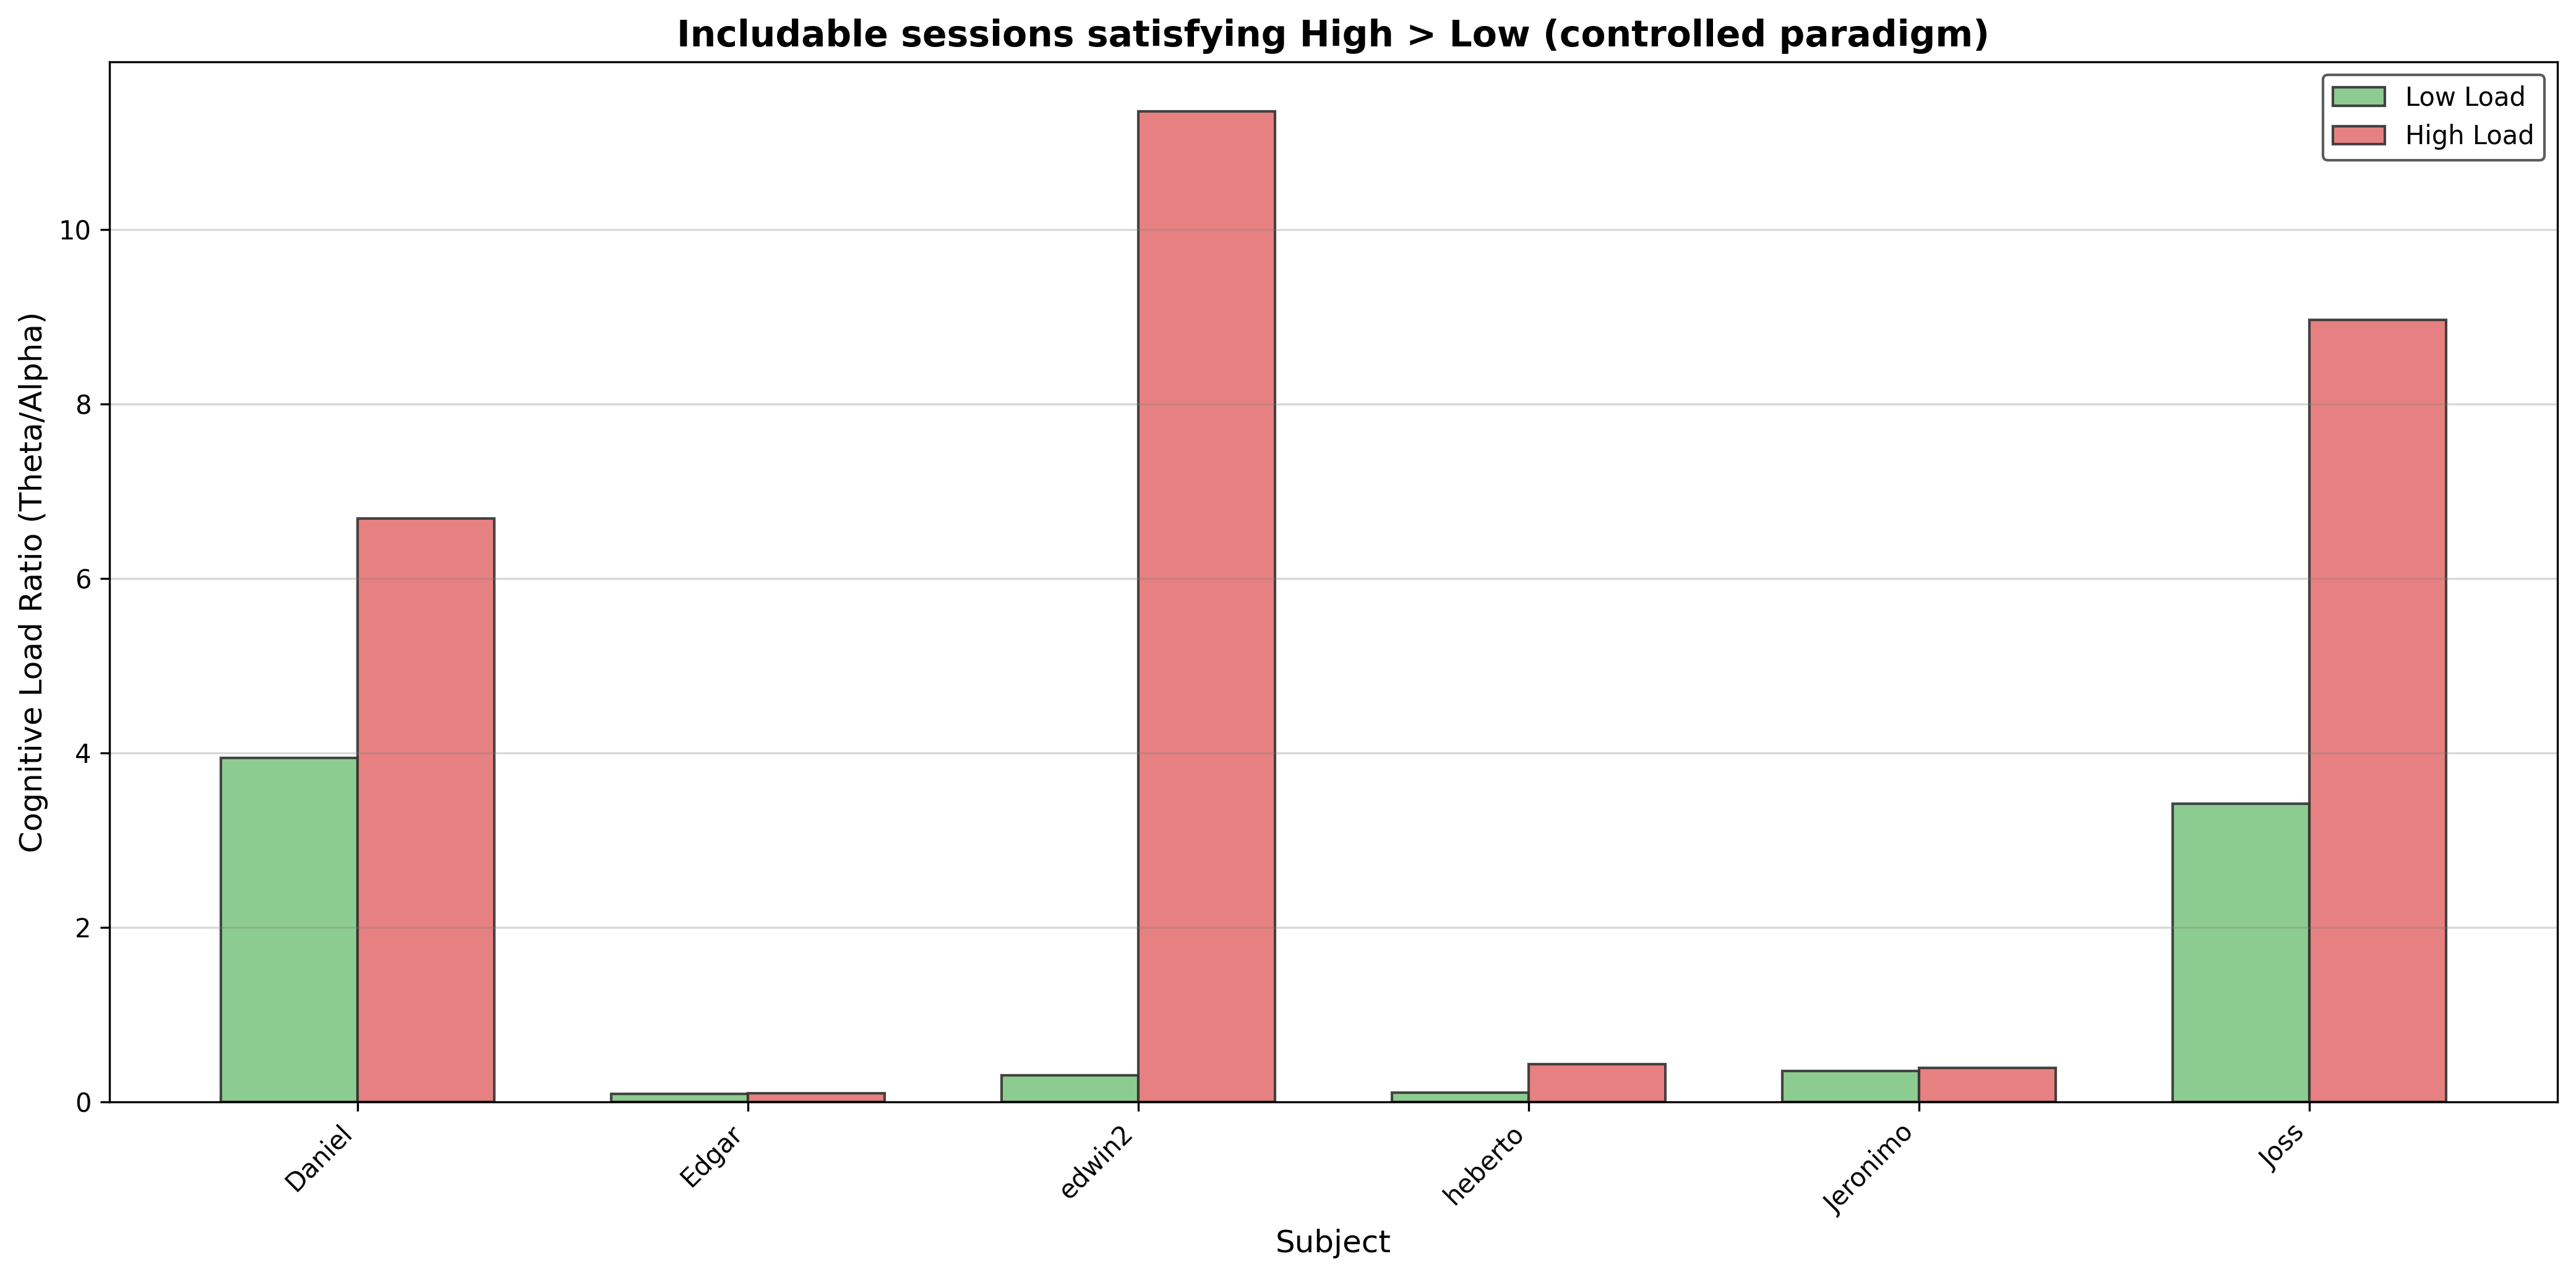
\includegraphics[width=\linewidth]{figures/cumplen_incluibles_ratios_absolutos.png}
\caption{Per-session theta/alpha ratio in Low Load vs. High Load for the six includable sessions (controlled paradigm).}
\label{fig:bars}
\end{figure}



\subsection{Ecological Paradigm: Exergaming Task (Baseline-Normalized)}

For the ecological exergaming paradigm, analysis was performed at the session level using recordings that contained an identifiable task segment (seg) suitable for comparison against baseline. The theta/alpha ratio was computed using the same index definition (Fz/Pz) and was normalized by each participant's baseline ratio:
\[
\mathrm{Index}_{\mathrm{norm}} = \frac{\mathrm{Index}_{\mathrm{task}}}{\mathrm{Index}_{\mathrm{baseline}}}.
\]
Normalized values greater than 1 indicate higher index values during the task segment relative to baseline.

Across 8 sessions containing a task segment, 6 sessions showed $\mathrm{Index}_{\mathrm{norm}} > 1$ (task $>$ baseline) and 2 sessions showed $\mathrm{Index}_{\mathrm{norm}} < 1$ (task $<$ baseline). The sessions with $\mathrm{Index}_{\mathrm{norm}} > 1$ exhibited normalized ratios of 7.85, 1.87, 2.51, 3.14, 4.08, and 2.14, respectively, whereas the remaining two sessions showed normalized ratios of 0.71 and 0.33.

Table~\ref{tab:eco} reports the baseline-normalized theta/alpha ratio during the task segment (seg) for each of the eight sessions. Session identifiers (S1--S8) correspond to individual recording sessions and do not necessarily represent unique participants, as some participants completed multiple sessions using different interaction modalities. The two sessions with normalized ratio below unity may reflect individual differences, baseline selection, or task engagement, and are not overinterpreted.
\begin{table}[H]
\centering
\caption{\textbf{Ecological paradigm: baseline-normalized theta/alpha ratio during the task segment (seg).}}
\label{tab:eco}
\footnotesize
\setlength{\tabcolsep}{6pt}
\begin{tabular}{lc}
\toprule
\textbf{Session} & \textbf{Normalized ratio (seg)} \\
\midrule
S1 & 7.85 \\
S2 & 1.87 \\
S3 & 2.51 \\
S4 & 3.14 \\
S5 & 4.08 \\
S6 & 2.14 \\
S7 & 0.71 \\
S8 & 0.33 \\
\bottomrule
\end{tabular}
\end{table}

\subsection{Subjective Workload Results and Convergent Trends}

NASA-TLX global scores increased consistently from the Low Load (passive reading) condition to the High Load (Stroop interference) condition across includable sessions, indicating higher perceived cognitive workload during the interference task. This subjective increase was directionally consistent with the EEG-based theta/alpha ratio, which also showed systematic increases under high cognitive demand.

Although formal correlation analysis was not performed due to the limited number of includable sessions, the parallel increase observed in both NASA-TLX scores and theta/alpha ratios supports the convergent validity of the EEG-based index as a marker of cognitive load under controlled conditions.

Mean NASA-TLX global scores (\%, $N=10$) were 48.8 (SD = 13.5) for the controlled paradigm (overall session), and 41.4 (SD = 14.1), 35.3 (SD = 13.8), and 44.1 (SD = 15.2) for the CanineQuest Haptic, Gamepad, and Keyboard interaction modalities, respectively. Among the three interface conditions, the Gamepad modality exhibited the lowest subjective workload on average.


\begin{table}[H]
\centering
\caption{\textbf{NASA-TLX subjective workload (\%): mean $\pm$ SD by condition (N=10).}}
\label{tab:nasa_tlx}
\begin{tabular}{lc}
\toprule
\textbf{Condition} & \textbf{Mean $\pm$ SD (\%)} \\
\midrule
Controlled paradigm (overall) & 48.8 $\pm$ 13.5 \\
CaniQuest Haptic & 41.4 $\pm$ 14.1 \\
CaniQuest Gamepad & 35.3 $\pm$ 13.8 \\
CaniQuest Keyboard & 44.1 $\pm$ 15.2 \\
\bottomrule
\end{tabular}
\end{table}
    
%%%%%%%%%%%%%%%%%%%%%%%%%%%%%%%%%%%%%%%%%%%%%%%%%%%%%%%%%%%%%%%%%%%%%%%%%%%%%%%%
\section{DISCUSSION}

The present study evaluated the theta/alpha ratio computed from frontal and parietal EEG channels (Fz/Pz) as an index of cognitive load across two complementary paradigms. In the controlled laboratory setting, the index consistently discriminated between low cognitive load (passive reading) and high cognitive load (Stroop interference) in all includable sessions, yielding a medium effect size at the group level. This finding aligns with recent evidence showing that ratios combining frontal theta and parietal alpha activity provide a compact and sensitive representation of mental workload~\cite{c1,c3,c7}.

The observed increase in the theta/alpha ratio during the Stroop task is consistent with contemporary interpretations of frontal theta as a marker of executive control and conflict monitoring, coupled with alpha suppression reflecting increased task engagement. Recent EEG studies of Stroop and related interference paradigms have reported similar spectral patterns, reinforcing the suitability of this task as a benchmark for validating cognitive load indices~\cite{c5,c9}. Importantly, the present results were obtained using a predefined preprocessing and artifact-handling pipeline, addressing concerns raised in recent methodological studies regarding the reproducibility and reliability of EEG-based workload metrics~\cite{c4,c6}.

Beyond the controlled paradigm, the ecological exergaming task provided an opportunity to explore the behavior of the same index in a less constrained and more interactive context. In the majority of analyzed sessions, the baseline-normalized theta/alpha ratio increased during the task segment, suggesting that the index is sensitive to cognitive demands in naturalistic interaction scenarios. This observation is in line with recent studies reporting EEG workload modulation during immersive and game-based tasks, where engagement and task demands fluctuate dynamically~\cite{c2,c3}. However, variability across sessions was also observed, with a subset of sessions showing lower normalized ratios relative to baseline.

Such variability is not unexpected in ecological paradigms and may reflect individual differences in baseline selection, task engagement, learning effects, or interaction modality. Recent literature emphasizes that cognitive load indices derived from EEG should be interpreted cautiously in unconstrained environments and are best complemented by normalization strategies and session-level analysis rather than strict subject-level inference~\cite{c1,c6}. In this context, the present findings support the sensitivity—but not uniform monotonicity—of the theta/alpha ratio in ecological settings.

Several limitations should be acknowledged. First, the number of includable sessions in the controlled paradigm was limited by strict signal-quality criteria, resulting in a modest sample size. Second, the ecological analysis was conducted at the session level without applying the same exclusion thresholds, which precludes direct statistical comparison with the controlled results. Finally, the use of short analysis windows, while suitable for temporal resolution, may increase variance in spectral estimates for sessions with limited valid data.

Future work will focus on expanding the dataset, incorporating graded task difficulty levels, and evaluating adaptive or real-time implementations of the theta/alpha index. In particular, integrating this index into closed-loop systems and multimodal frameworks, as suggested in recent workload monitoring studies~\cite{c10}, represents a promising direction for bridging controlled validation and applied neuroergonomic applications.

\section{Materials to consider for the ADHD K9 Canine Quest exergaming}
%
The development of emerging technologies has transformed clinical intervention strategies for neurodivergent populations, enabling novel tools that enhance both diagnostic accuracy and therapeutic efficacy. When combined with convergent approaches, these technologies facilitate the integration of disciplines such as neuroscience, biomedical engineering, and clinical psychology, thereby maximizing their translational and therapeutic impact. Exergames have emerged as effective convergent technologies for stimulating neurocognitive functions in children with ADHD by combining physical activity with game-based mechanics that enhance attention, working memory, and inhibitory control ~\cite{14, 15}. ADHD K9 Canine Quest, developed at the Advanced Robotics and Haptic Interfaces Laboratory (UAEH), is an exergame specifically designed to integrate a human–robotic interaction (HRpI) system with haptic feedback and eye-tracking, enabling the training and assessment of executive functions within an immersive and personalized environment ~\cite{16}. Recent evidence suggests that such interventions can induce measurable changes in functional brain connectivity and neural plasticity, supporting cognitive and emotional development in this population ~\cite{17}.

\begin{figure}[htbp]
    \begin{subfigure}{.47\textwidth}
        \centering
        
\includegraphics[width=\linewidth]{figures/CQuest1.jpg}
        \caption{Virtual reality environment for assessment.}
        \label{CQuest1}
    \end{subfigure}\hfill
    %
    \begin{subfigure}{.47\textwidth}
        \centering
        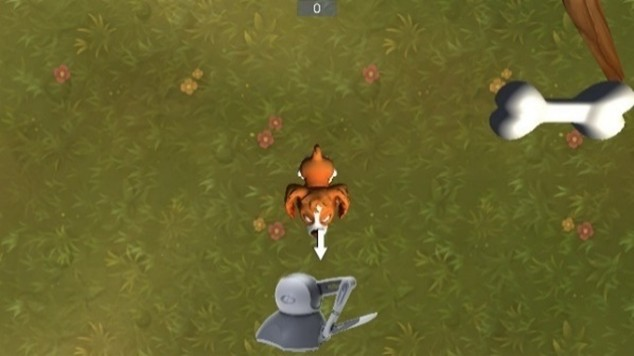
\includegraphics[width=\linewidth]{figures/CQuest2.jpg}
        \caption{Haptic interface for exploration.}
        \label{CQuest2}
    \end{subfigure}\hfill
    %
    \begin{subfigure}{.47\textwidth}
        \centering
        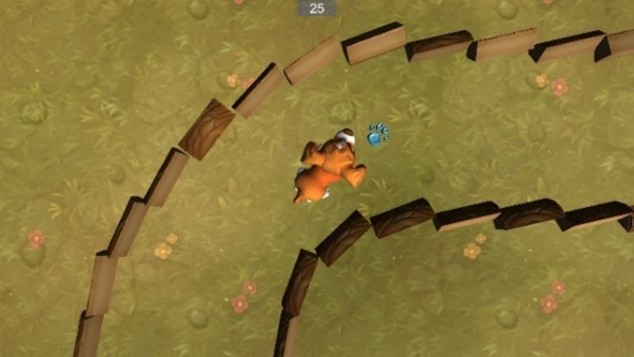
\includegraphics[width=\linewidth]{figures/CQuest4.jpg}
        \caption{User evaluation of the exploration.}
        \label{CQuest4}
    \end{subfigure}
    \caption{ADHD K9 Canine Quest Exergaming.}
    \label{Exergaming}
\end{figure}



\subsection{Implementation and Validation of a Neurophysiological Biofeedback Protocol for Cognitive Performance Optimization}

Biofeedback (BF) is a therapeutic and training approach that enables individuals to acquire voluntary control over physiological processes typically governed by autonomic regulation, including cardiac activity, respiration, peripheral temperature, and cortical electrical activity. In EEG-based biofeedback, real-time neurophysiological markers are feedback to the user, facilitating self-regulation of brain states associated with cognitive and emotional processes. When embedded within interactive and game-based environments such as exergames, BF can enhance user engagement and ecological validity while supporting adaptive modulation of cognitive load. In clinical applications, particularly for attention-deficit/hyperactivity disorder (ADHD), EEG-biofeedback interventions have shown promising effects on attentional control and emotional regulation, supporting their use as complementary tools for cognitive performance optimization ~\cite{18}.

\subsection{Haptic interface applied in the exergame}

The haptic device consists of an articulated-link mechanism designed to deliver tactile and kinesthetic neurostimulation by engaging cutaneous mechanoreceptors, proprioceptors, and kinesthetic pathways. It enables bidirectional human interaction with virtual environments by providing force feedback that supports kinesthetic perception through muscles, tendons, and joints. The dynamics of the virtual reality environment are modeled to reproduce realistic interaction conditions via controlled force rendering. This technology supports two primary modes of interaction: active haptic exploration and passive haptic guidance. In active haptic exploration, users voluntarily control their movements to interact with the device, promoting autonomous learning through trial-and-error mechanisms, while the virtual environment dynamically responds to user input. In contrast, passive haptic guidance involves the intervention of an external agent—such as a human trainer or an autonomous robotic system—that constrains or guides the user’s movements during task execution (e.g., within a clinical training protocol), thereby enhancing movement accuracy and potentially reducing cognitive load ~\cite{22, 23}.

\begin{figure*}[]
    \centering
    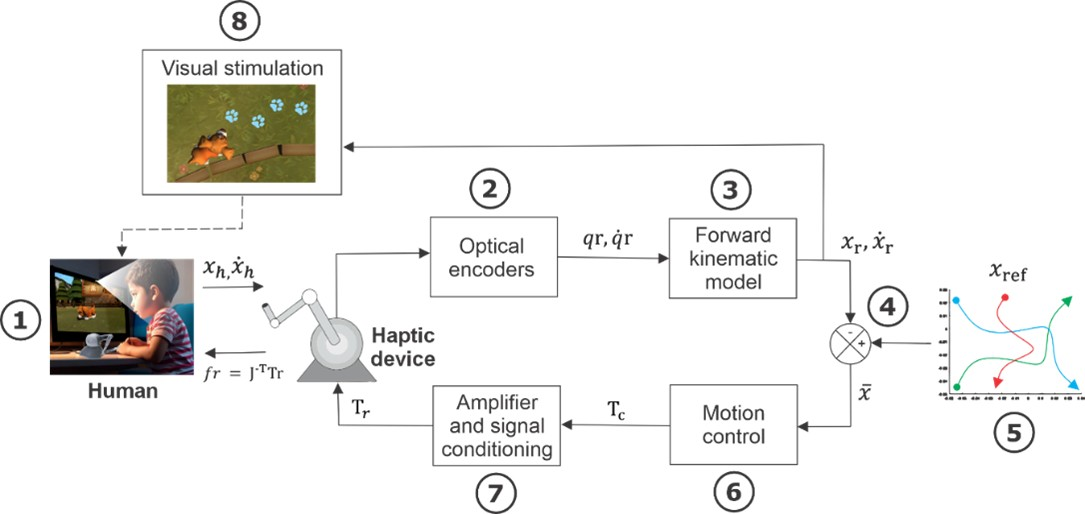
\includegraphics[width=1\linewidth]{figures/CQuest3.jpg}
    \caption{Passive haptic guidance scheme for training purposes. }
    \label{CQuest3}
\end{figure*}


%%%%%%%%%%%%%%%%%%%%%%%%%%%%%%%%%%%%%%%%%%%%%%%%%%%%%%%%%%%%%%%%%%%%%%%%%%%%%%%%
\section{Conclusion}
Under a controlled baseline--low--high protocol, the theta/alpha ratio computed from Fz and Pz discriminated passive reading from Stroop interference in six subjects satisfying predefined data-quality criteria. The increase from 1.37 (SD=1.80) to 4.65 (SD=4.99) and the paired Cohen's $d=0.75$ support the theta/alpha ratio (Fz/Pz) as a practical index for cognitive load validation in controlled experiments.

%%%%%%%%%%%%%%%%%%%%%%%%%%%%%%%%%%%%%%%%%%%%%%%%%%%%%%%%%%%%%%%%%%%%%%%%%%%%%%%%
\section*{ACKNOWLEDGMENT}
The authors thank the Mirai Innovation Research Institute team for their support and for providing the AURA EEG acquisition system and the experimental infrastructure.\textcolor{blue}{The first two authors acknowledge the Secretariat of Science, Humanities, Technology and Innovation (SECIHTI), Mexico, for the doctoral scholarships received. The third author acknowledges support from the National System of Researchers (SNII) of SECIHTI, Mexico.}

%%%%%%%%%%%%%%%%%%%%%%%%%%%%%%%%%%%%%%%%%%%%%%%%%%%%%%%%%%%%%%%%%%%%%%%%%%%%%%%%
\begin{thebibliography}{99}

\bibitem{c1}
B. Raufi and L. Longo, ``An Evaluation of the EEG Alpha-to-Theta and Theta-to-Alpha Band Ratios as Indexes of Mental Workload,'' \emph{Frontiers in Neuroinformatics}, Vol. 16, p. 861967, 2022. \hl{https://doi.org/10.3389/fninf.2022.861967}

\bibitem{c2}
R. Khan, A. R. B. Manzoor, and A. Leitão, ``Assessing cognitive load using EEG and eye-tracking in immersive environments,'' \emph{Multimodal Technologies and Interaction}, vol. 9, no. 9, p. 99,  

\bibitem{c3}
A. D. Blanco et al., ``EEG spectral power correlates across cognitive tasks with Theta-to-Alpha Ratio (TAR) significance,'' \emph{Journal of Neuroscience Methods}, vol. [to be filled], 2025. 

\bibitem{c4}
S. Chikhi, N. Matton, and S. Blanchet, ``EEG power spectral measures of cognitive workload: A meta-analysis,'' \emph{Psychophysiology}, vol. 59, no. 6, p. e14009, 2022. 

\bibitem{c5}
M. Pušica et al., ``Machine learning performance in EEG-based mental workload estimation and frontal midline theta activity,'' \emph{Frontiers in Neuroergonomics}, vol. [to be filled], 2025. 

\bibitem{c6}
M. Mondellini and S. Caggiula, ``A multimodal approach exploiting EEG to investigate mental workload,'' \emph{International Journal of Human-Computer Studies}, vol. [to be filled], 2024. 

\bibitem{c7}
S. Moontaha and A. Mathew, ``Wearable EEG-based cognitive load classification using spectral band ratios,'' \emph{Brain Sciences}, vol. [to be filled], 2023. 

\bibitem{c8}
E. Khan, J. Maguire, and D. Schneider, ``Theta activity and cognitive functioning: Task-related increases in frontal theta during cognitive demand,'' \emph{Cognitive Neuroscience}, vol. [to be filled], 2024. 

\bibitem{c9}
J. Wu et al., ``Brain functional connectivity changes induced by cognitive tasks including Stroop: Evidence from EEG/fMRI studies,'' \emph{Scientific Reports}, vol. [to be filled], 2025. 

\bibitem{c10}
A. Arana-De-Las Casas et al., ``Real-time mental workload measurement for cognitive tasks using an EEG-based workload index,'' Research Report, 2024. 

\bibitem {14}
A. Serrano-Barroso et al., “Detecting attention levels in ADHD children with a video game and the measurement of brain activity with a single-channel BCI headset,” Sensors, vol. 21, no. 9, p. 3221, 2021.

\bibitem {15}
H. Ji et al., “The Effects of Exergaming on Attention in Children With Attention Deficit/Hyperactivity Disorder: Randomized Controlled Trial,” JMIR Serious Games, vol. 11, p. e40438, May 2023, doi: 10.2196/40438.

\bibitem {16}
B. Tleubayev, Z. Zhexenova, A. Zhakenova, and A. Sandygulova, “Robot-assisted therapy for children with ADHD and ASD: A pilot study,” ACM Int. Conf. Proceeding Ser., pp. 58–62, 2019, doi: 10.1145/3325693.3325703.

\bibitem {17}
M. Amin, A. Tubaishat, F. Al-Obeidat, B. Shah, and M. Karamat, “Leveraging brain-computer interface for implementation of a bio-sensor controlled game for attention deficit people,” Comput. Electr. Eng., vol. 102, p. 108277, 2022.

\bibitem {18} 
C. Argáez and S. Banerjee, “Neurofeedback and Biofeedback for Mood and Anxiety Disorders: A Review of Clinical Effectiveness and Guidelines,” 2017.

\bibitem {22} 
O. A. Dominguez-Ramirez and V. Parra-Vega, “Active haptic exploration of deformable objects,” en DAAAM International Scientific Book 2006, B. Katalinic, Ed., DAAAM International, 2006, pp. 177–190.

\bibitem {23} 
O. A. Dominguez-Ramirez and V. Parra-Vega, “Texture, Roughness and Shape Haptic Perception of Deformable Virtual Objects with Constrained Lagrangian Formulation,” en IEEE/RSJ International Conference on Intelligent Robots and Systems, Proceedings of IROS, 2003.




\textcolor{red}{Debemos considerar las direcciones DOI de cada artículo citado.}



\end{thebibliography}




\end{document}
